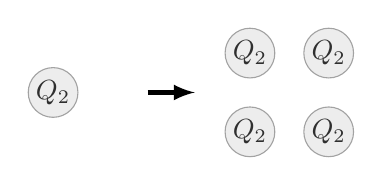
\begin{tikzpicture}[>=latex]
\def\Length{1}
\def\Radius{0.07}

% pre refinement
\LagrangeCell{0}{0}{2*\Length}{\Radius}{2}
  {{,,,,,,,,}};
\node[circle, draw=gray, fill=gray!20, inner sep=1pt, opacity=0.7, text opacity=0.8] at (\Length,\Length) {$Q_2$};

% arrow
\draw[->,ultra thick] (2.2*\Length,\Length) -- (2.8*\Length,\Length);

% post refinement
\LagrangeCell{3*\Length}{0}{\Length}{\Radius}{2}
  {{,,,,,,,,}};
\node[circle, draw=gray, fill=gray!20, inner sep=1pt, opacity=0.7, text opacity=0.8] at (3.5*\Length,0.5*\Length) {$Q_2$};

\LagrangeCell{4*\Length}{0}{\Length}{\Radius}{2}
  {{,,,,,,,,}};
\node[circle, draw=gray, fill=gray!20, inner sep=1pt, opacity=0.7, text opacity=0.8] at (4.5*\Length,0.5*\Length) {$Q_2$};

\LagrangeCell{3*\Length}{\Length}{\Length}{\Radius}{2}
  {{,,,,,,,,}};
\node[circle, draw=gray, fill=gray!20, inner sep=1pt, opacity=0.7, text opacity=0.8] at (3.5*\Length,1.5*\Length) {$Q_2$};

\LagrangeCell{4*\Length}{\Length}{\Length}{\Radius}{2}
  {{,,,,,,,,}};
\node[circle, draw=gray, fill=gray!20, inner sep=1pt, opacity=0.7, text opacity=0.8] at (4.5*\Length,1.5*\Length) {$Q_2$};
\end{tikzpicture}